\documentclass{article}
\usepackage[T1]{fontenc}
\usepackage[polish]{babel}
\usepackage[utf8]{inputenc}
\usepackage{graphicx}
\graphicspath{{images/}}
\usepackage{blindtext}
\usepackage{hyperref}

\title{Generacja tekstów piosenek}
\author{Maciej Krzyżanowski, Sebastian Kutny, Tomasz Lewandowski}
\date{Kwiecień 2023}

\begin{document}

\maketitle

\tableofcontents

\newpage
\section{Wstęp}
Celem projektu było stworzenie modelu generującego tekst piosenki na podstawie wybranych danych jako tekstów innych utworów. Wykorzystaliśmy 2 metody: łańcuchy Markova oraz rekurencyjne sieci neuronowe. \\ \\ Projekt zawiera narzędzie "scraper" do pozyskiwania danych ze stron: 
\begin{itemize}
    \item \url{https://www.tekstowo.pl}
    \item \url{https://www.azlyrics.com}
\end{itemize}
Implementacja została wykonana w języku Python oraz wykorzystuje biblioteki: 
\begin{itemize}
    \item pandas
    \item BeautifulSoup
    \item nltk
    \item request
    \item queue
    \item re
\end{itemize}
Dostępna jest opcja łączenia zbiorów danych do jednego pliku w celu wykorzystania ich jednocześnie. \\ \\
Przed rozpoczęciem przetwarzania danych są one oczyszczane poprzez ujednolcenie wielkości liter, usunięcie niepotrzebnych znaków interpunkcyjnych, słów zakazanych (np:. określających składowe tekstu utworu) oraz wyrażeń ze szczególnymi znakami interpunkcyjnymi jako określających zawartość tekstu.
\\ \\
Tekst jest generowany jako dowolna liczba wersów o dowolnej ilości słow.
\newpage
\section{Łańcuchy Markova}
Łańcuchy Markova to matematyczny model służący do generowania tekstu lub sekwencji innych elementów, takich jak dźwięki lub obrazy. Ideą modelu jest analiza sekwencji istniejących elementów i wykorzystanie tych informacji do przewidywania, jakie elementy powinny pojawić się następnie. \\
\\
W przypadku generowania tekstu, łańcuchy Markova są zwykle stosowane do analizy sekwencji słów w tekście źródłowym i generowania nowych sekwencji słów na podstawie tych informacji. Proces zaczyna się od wyboru deterministycznego lub losowego początkowego stanu łańcucha, a następnie generowania kolejnych stanów na podstawie informacji o pradwopodobieństwie wystąpienia po sobie stanów w analizowanym tekście w kontekście poprzednio wygenerowanych stanów. Przykładowo, jeśli w tekście źródłowym po słowie "generator" często pojawia się słowo "piosenek", to model łańcucha Markova przypisze wysokie prawdopodobieństwo wystąpienia słowa "piosenek" po słowie "generator". \\
\\
Istnieją różne sposoby implementacji modelu łańcuchów Markova, ale zwykle opierają się one na analizie pewnej liczby poprzednich elementów, zwanej "stopniem" modelu. Na przykład, w przypadku modelu pierwszego stopnia, prawdopodobieństwo wystąpienia danego elementu zależy tylko od poprzedniego elementu, w modelu drugiego stopnia, prawdopodobieństwo zależy od dwóch poprzednich elementów, a w modelu trzeciego stopnia, prawdopodobieństwo zależy od trzech poprzednich elementów itd. Stopień łańcucha nazywamy N-gramem.\\
\\
W naszym projektcie N-gram jest parametryzowany i bazuje na N uprzednio wygenerowanych słowach w wersie, losując następne słowo na podstawie prawdopodobieństwa jego wystąpienia po N sekwencji słów uprzednio wygenerowanych. Dodatkowo przy każdym wersie o nieparzystym numerze podejmowana jest próba stworzenia rymującego się wersu na podstawie ostatniej sylaby poprzedniego. Najpierw znajdowane są wszystkie rymujące się zakończenia wersu niebędące ostatnim słowem poprzedniego, a następnie - jeśli takie istnieją - losujemy jedno z nich zamiast z wszyskich pozycji. Przy nieznalezieniu rymujących się słów generacja odbywa się tak jak w zwykłym wypadku. W praktyce szansa na stworzenie rymu jest mała i powinna rosnąć z ilością danych przetwarzanych przez model.\\
\\
Model łańcuchów Markova nie jest idealny i może generować sekwencje, które nie są sensowne lub poprawne gramatycznie. Dopiero przy wglądzie modeli w setki stanów wstecz oraz przy bardzo dużej ilości danych można wygenerować tekst podobny do pisanego przez człowieka. \\
\\
\begin{figure}[h]
    \centering
    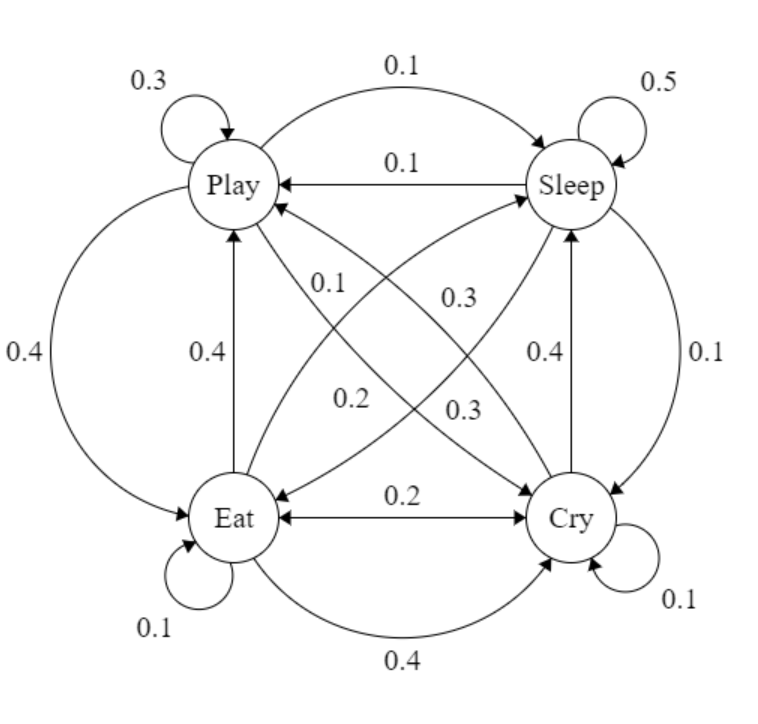
\includegraphics[width=0.75\textwidth]{plot}
    \caption{Przykład łańcucha Markova, gdzie stany mogą oznaczać słowa lub sekwencje słów, a przejścia pomiędzy nimi określono jako prawdpopodobieństwa $p$}
    \label{fig:mesh1}
\end{figure}

\newpage
\section{Rekurencyjne Sieci Neuronowe}
\end{document}
